\documentclass[aspectratio=169,11pt]{beamer}

\usepackage[T1]{fontenc}
\usepackage{lmodern}
\usepackage{amsmath,amssymb}
\usepackage{booktabs}
\usepackage{graphicx}
\usepackage{xcolor}

\graphicspath{{../Final_Report_Research/pic/generated/}}
\usetheme{Madrid}
\definecolor{researchblue}{RGB}{20,75,115}
\definecolor{researchteal}{RGB}{15,120,125}
\definecolor{researchorange}{RGB}{220,120,40}
\definecolor{softblue}{RGB}{232,242,249}
\definecolor{softred}{RGB}{252,236,236}
\setbeamercolor{structure}{fg=researchblue}
\setbeamercolor{palette primary}{bg=researchblue,fg=white}
\setbeamercolor{palette secondary}{bg=researchteal,fg=white}
\setbeamercolor{palette tertiary}{bg=researchblue!85!black,fg=white}
\setbeamercolor{frametitle}{bg=researchblue,fg=white}
\setbeamercolor{title}{fg=white}
\setbeamercolor{titlelike}{bg=researchblue,fg=white}
\setbeamercolor{block title}{bg=researchblue,fg=white}
\setbeamercolor{block body}{bg=softblue}
\setbeamercolor{block title alerted}{bg=researchorange,fg=white}
\setbeamercolor{block body alerted}{bg=softred}
\setbeamertemplate{navigation symbols}{}
\setbeamertemplate{bibliography item}[text]
\newcommand{\source}[1]{\vfill{\tiny\color{gray!80}Source: \cite{#1}}}
\newcommand{\figcaption}[1]{\vspace{0.08cm}{\scriptsize #1}}

\title[MLII ECG]{MLII ECG Anomaly Detection\\and Arrhythmia Classification}
\subtitle{Final one-lead temporal-holdout system}
\author[A.K.S.S. Wimalasena]{A.K.S.S. Wimalasena}
\institute[University of Ruhuna]{Department of Mathematics\\University of Ruhuna}
\date{Final Research Presentation -- August 2026}

\begin{document}

\begin{frame}[plain]
  \titlepage
  \vspace{-0.4cm}
  \begin{center}\small Supervisor: Ms. Sachini Karunarathne\end{center}
\end{frame}

\begin{frame}{The study makes two decisions from one ECG lead}
\begin{columns}[T,onlytextwidth]
\begin{column}{0.50\textwidth}
\begin{block}{Decision sequence}
\begin{enumerate}
  \item Detect whether the current MLII beat is normal or abnormal.
  \item If abnormal, classify PVC, PAC, LBBB, RBBB, or AFib.
\end{enumerate}
\end{block}
\end{column}
\begin{column}{0.46\textwidth}
\begin{alertblock}{Claim boundary}
The result measures later ECG from known MITDB patients. It is not an
unseen-patient or external-hospital validation.
\end{alertblock}
\end{column}
\end{columns}
\vspace{0.28cm}
The target was more than 90\% whole-system accuracy, with a subject-clustered
95\% confidence interval whose lower bound also exceeds 90\%.
\source{dechazal2004heartbeat,moody2001impact}
\end{frame}

\begin{frame}{The problem is not a simple ECG-threshold task}
\centering
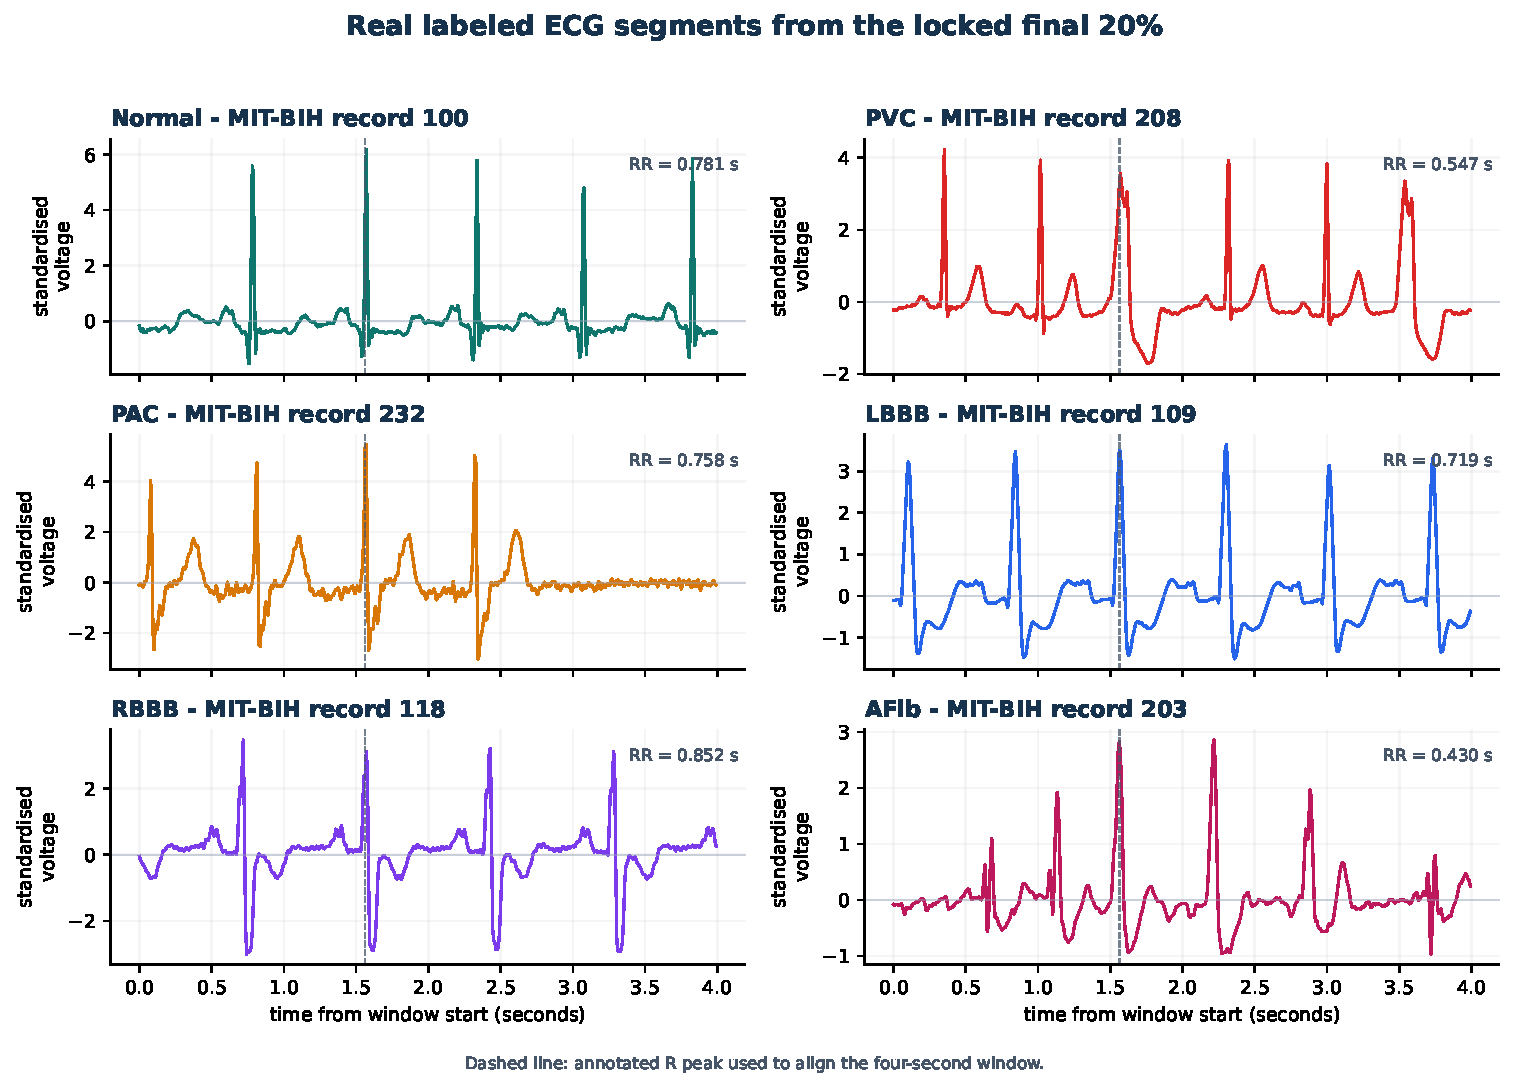
\includegraphics[width=0.96\textwidth,height=0.66\textheight,keepaspectratio]{real_arrhythmia_examples.pdf}

\figcaption{PVC, LBBB, and RBBB mainly alter morphology; PAC and AFib also
need rhythm context. The model therefore combines MLII shape, RR timing, and
normal-reconstruction mismatch.}
\source{mitdb}
\end{frame}

\begin{frame}{Normal-reference and arrhythmia data have separate roles}
\centering
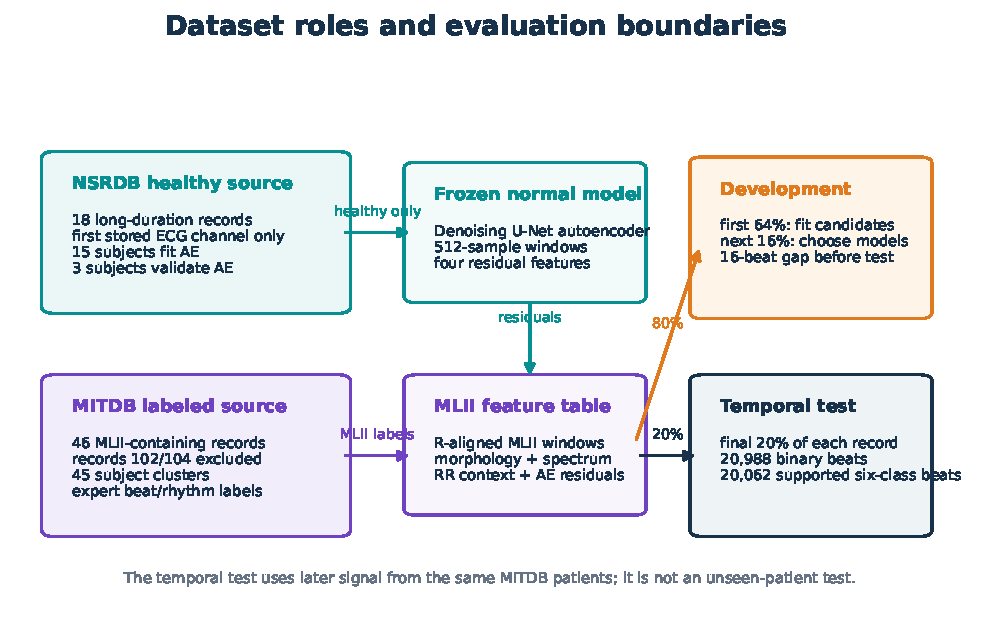
\includegraphics[width=0.93\textwidth,height=0.66\textheight,keepaspectratio]{dataset_role_overview.pdf}

\figcaption{NSRDB creates the frozen normal autoencoder. MITDB MLII creates
the supervised feature table and the final temporal test.}
\source{nsrdb,mitdb}
\end{frame}

\begin{frame}{The supervised system is strictly MLII-only}
\centering
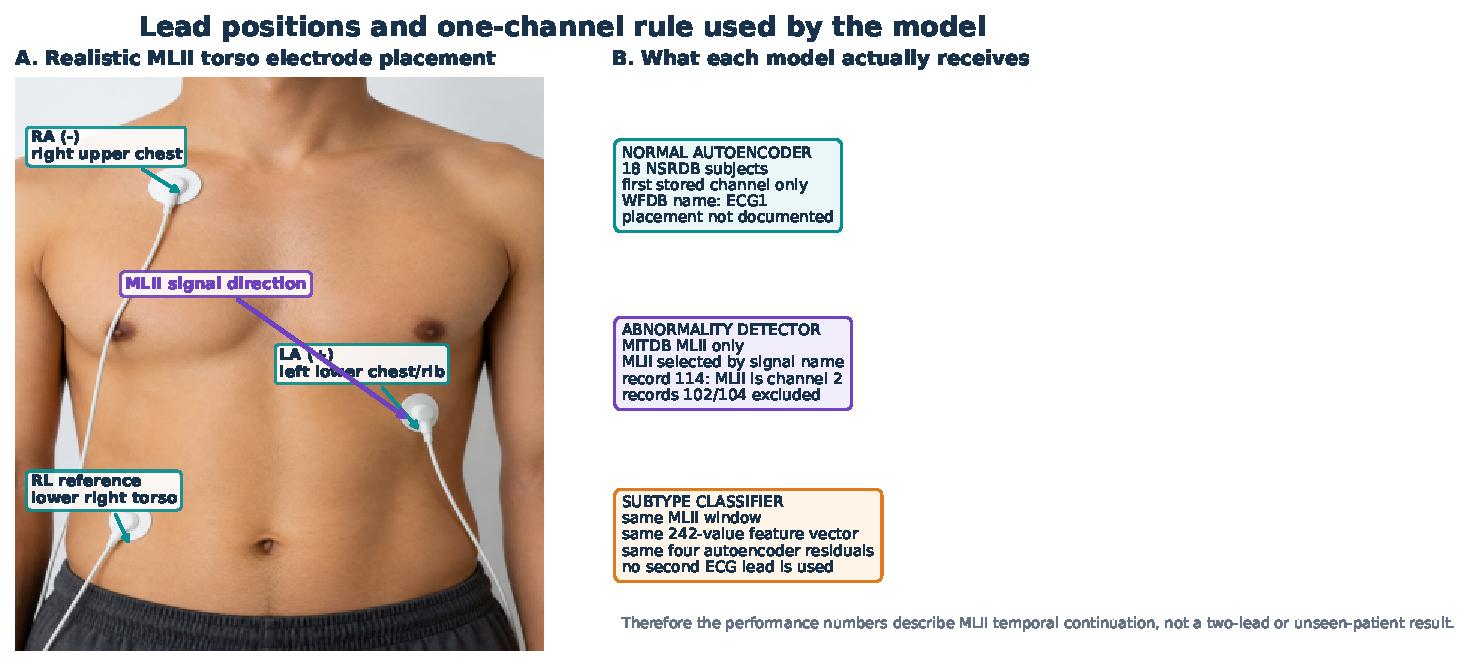
\includegraphics[width=0.94\textwidth,height=0.66\textheight,keepaspectratio]{real_lead_positions.pdf}

\figcaption{The autoencoder uses the first stored NSRDB ECG channel. The
detector, subtype classifier, temporal test, and installed replay use MLII
selected by signal name.}
\source{nsrdb,mitdb}
\end{frame}

\begin{frame}{Cleaning keeps the two signal roles explicit}
\centering
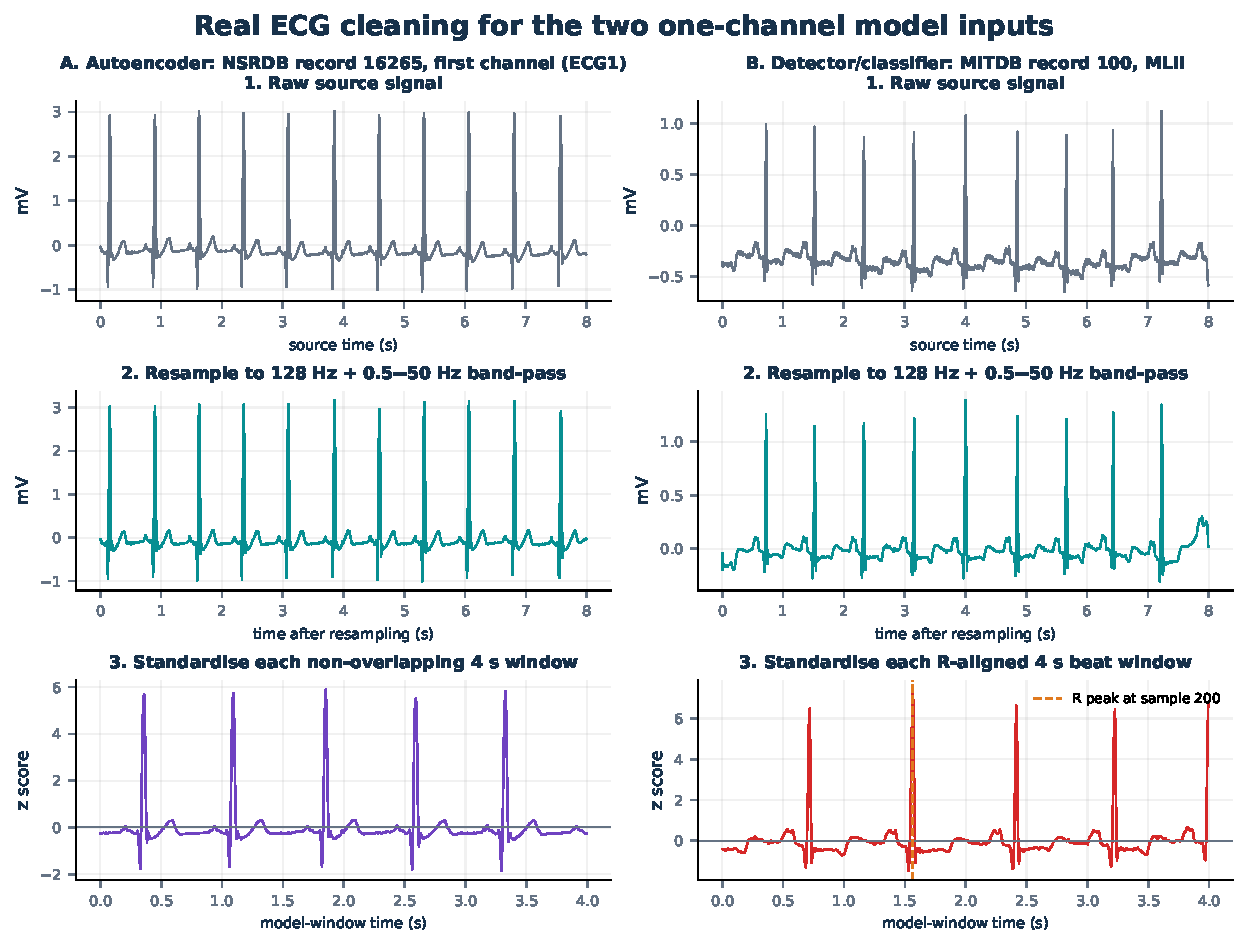
\includegraphics[width=0.92\textwidth,height=0.70\textheight,keepaspectratio]{real_data_cleaning_pipeline.pdf}

\figcaption{Both pipelines output one 512-sample input, but the healthy NSRDB
reference channel and the MITDB MLII deployment channel are not treated as
the same lead.}
\end{frame}

\begin{frame}{Training and use follow one fixed preparation route}
\centering
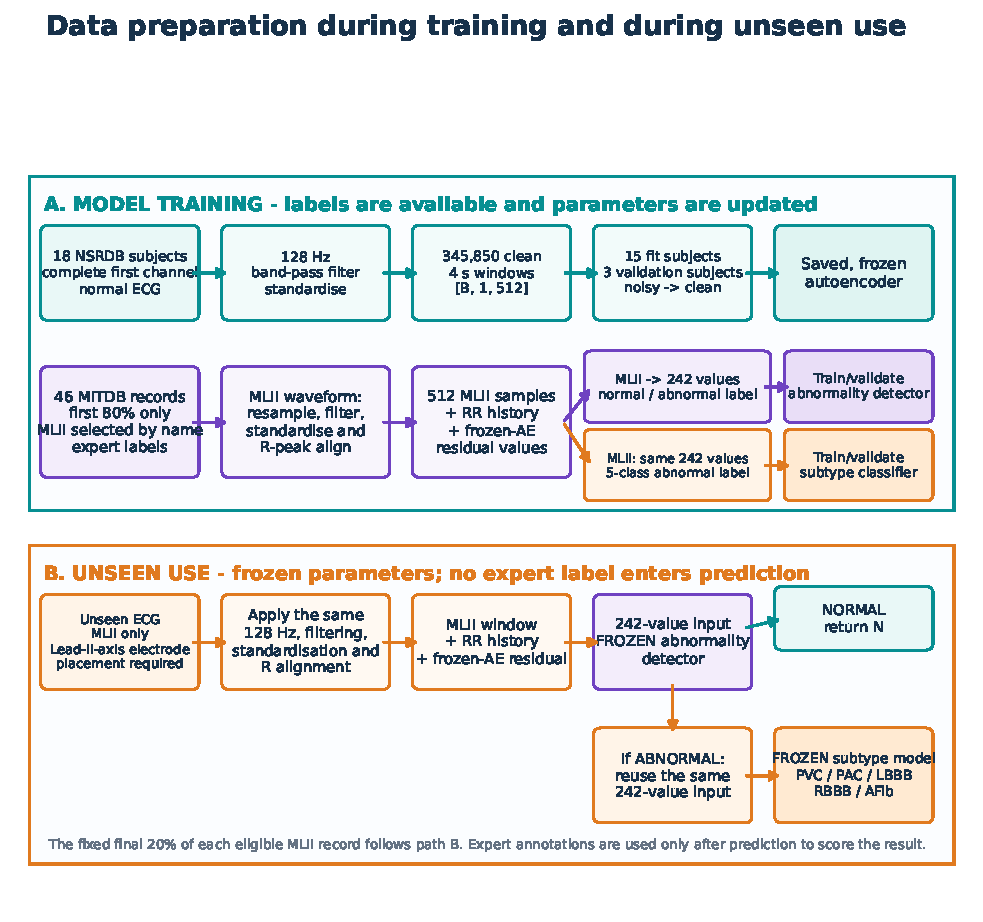
\includegraphics[width=0.91\textwidth,height=0.70\textheight,keepaspectratio]{real_data_preparation_flow.pdf}

\figcaption{The same resampling, filtering, standardisation, R alignment, RR
calculation, and feature order are used during development and installed use.}
\end{frame}

\begin{frame}{The model uses morphology and rhythm evidence together}
\centering
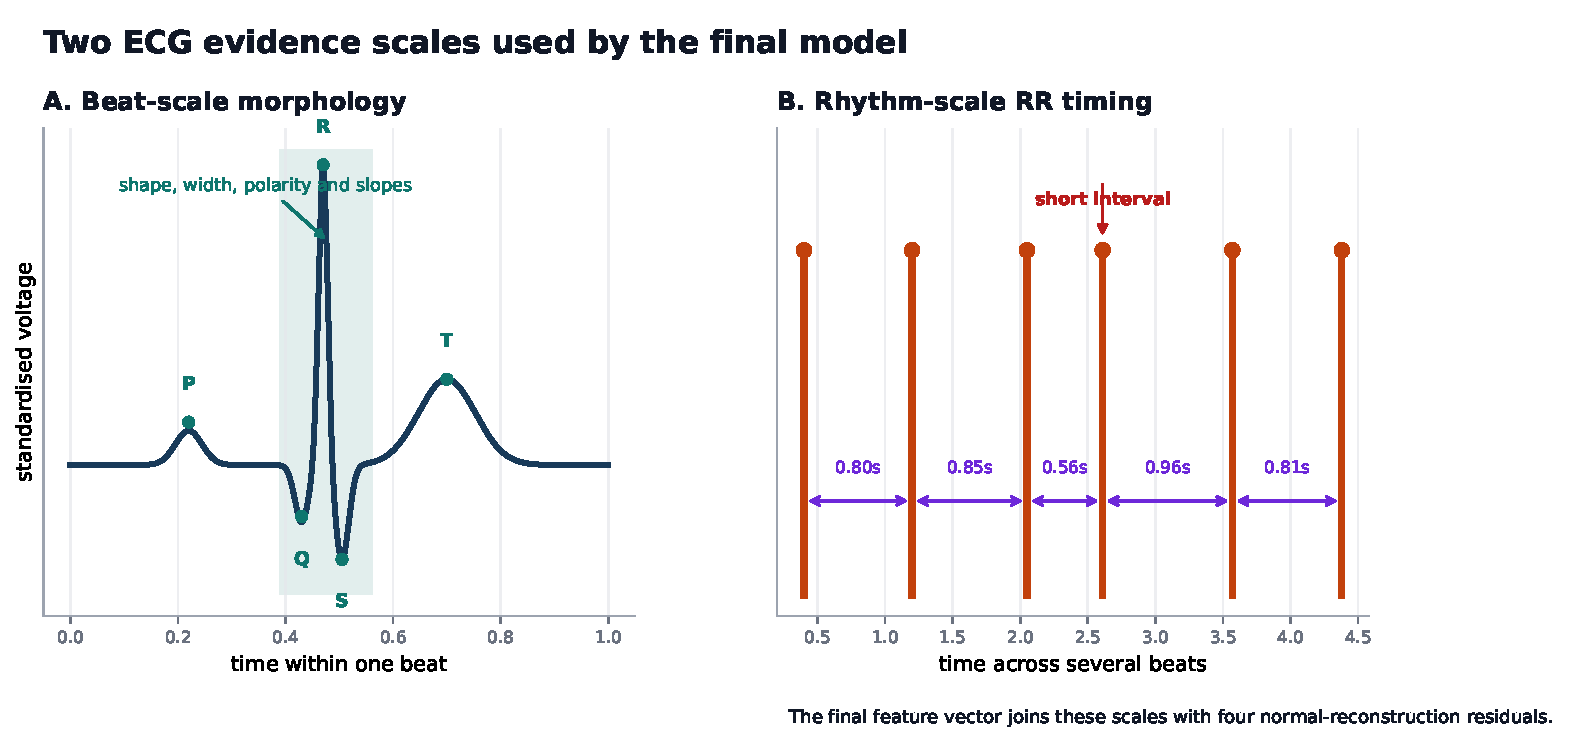
\includegraphics[width=0.94\textwidth,height=0.70\textheight,keepaspectratio]{theory_evidence_scales.pdf}

\figcaption{Morphology describes the local beat shape; RR timing describes
where that beat occurs in the rhythm sequence.}
\source{dechazal2004heartbeat,mousavi2019seq2seq}
\end{frame}

\begin{frame}{Raw ECG becomes compact numerical evidence}
\centering
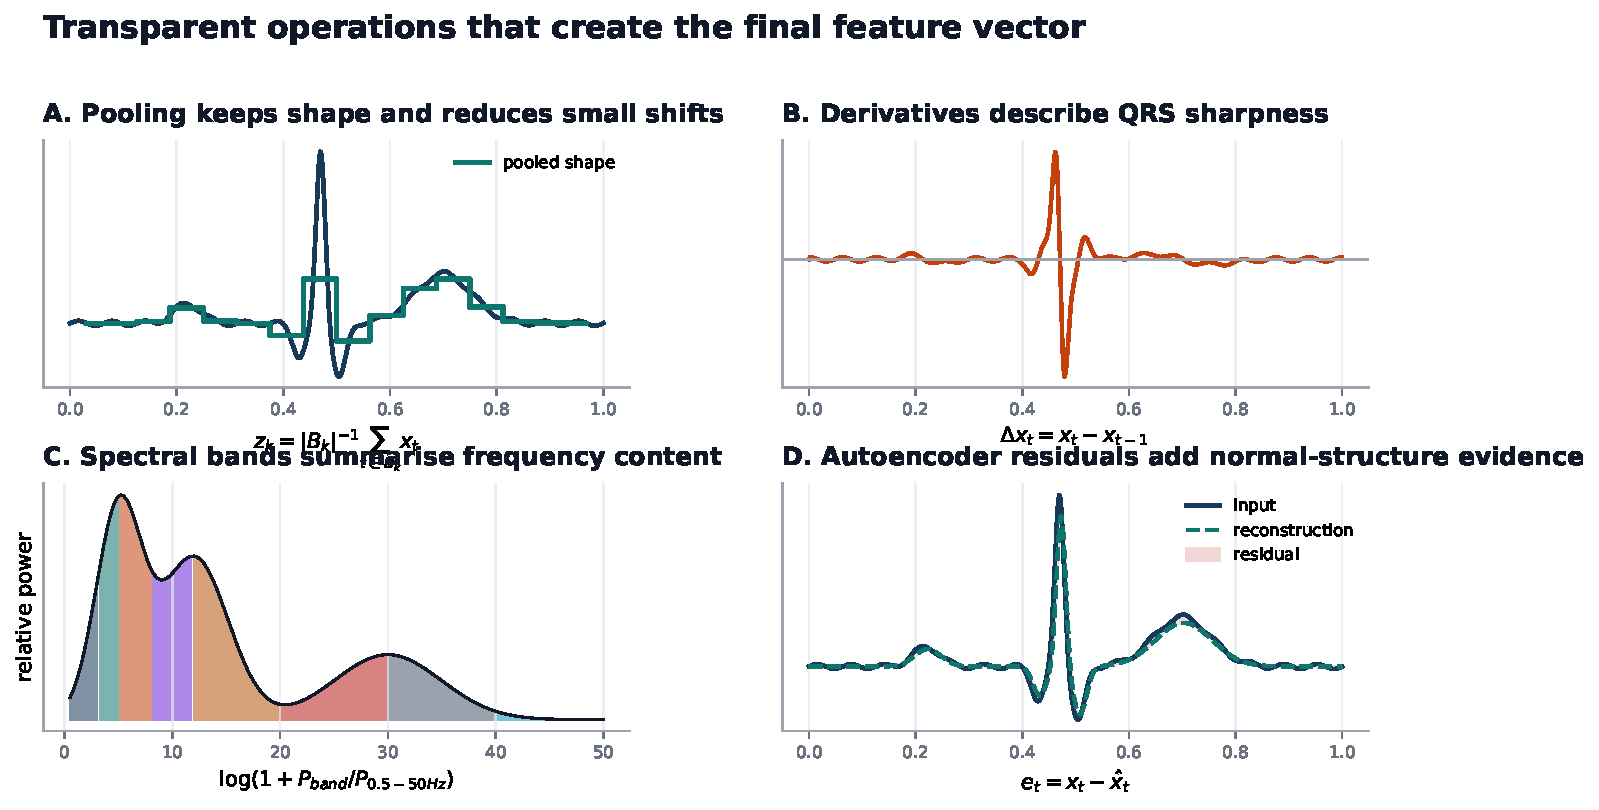
\includegraphics[width=0.93\textwidth,height=0.66\textheight,keepaspectratio]{theory_feature_math.pdf}

\figcaption{Pooling, derivatives, frequency power, and statistics preserve
useful MLII evidence while reducing sensitivity to small shifts and noise.}
\source{kligfield2007standardization,butterworth1930filter}
\end{frame}

\begin{frame}{Normal reconstruction is evidence, not the diagnosis}
\centering
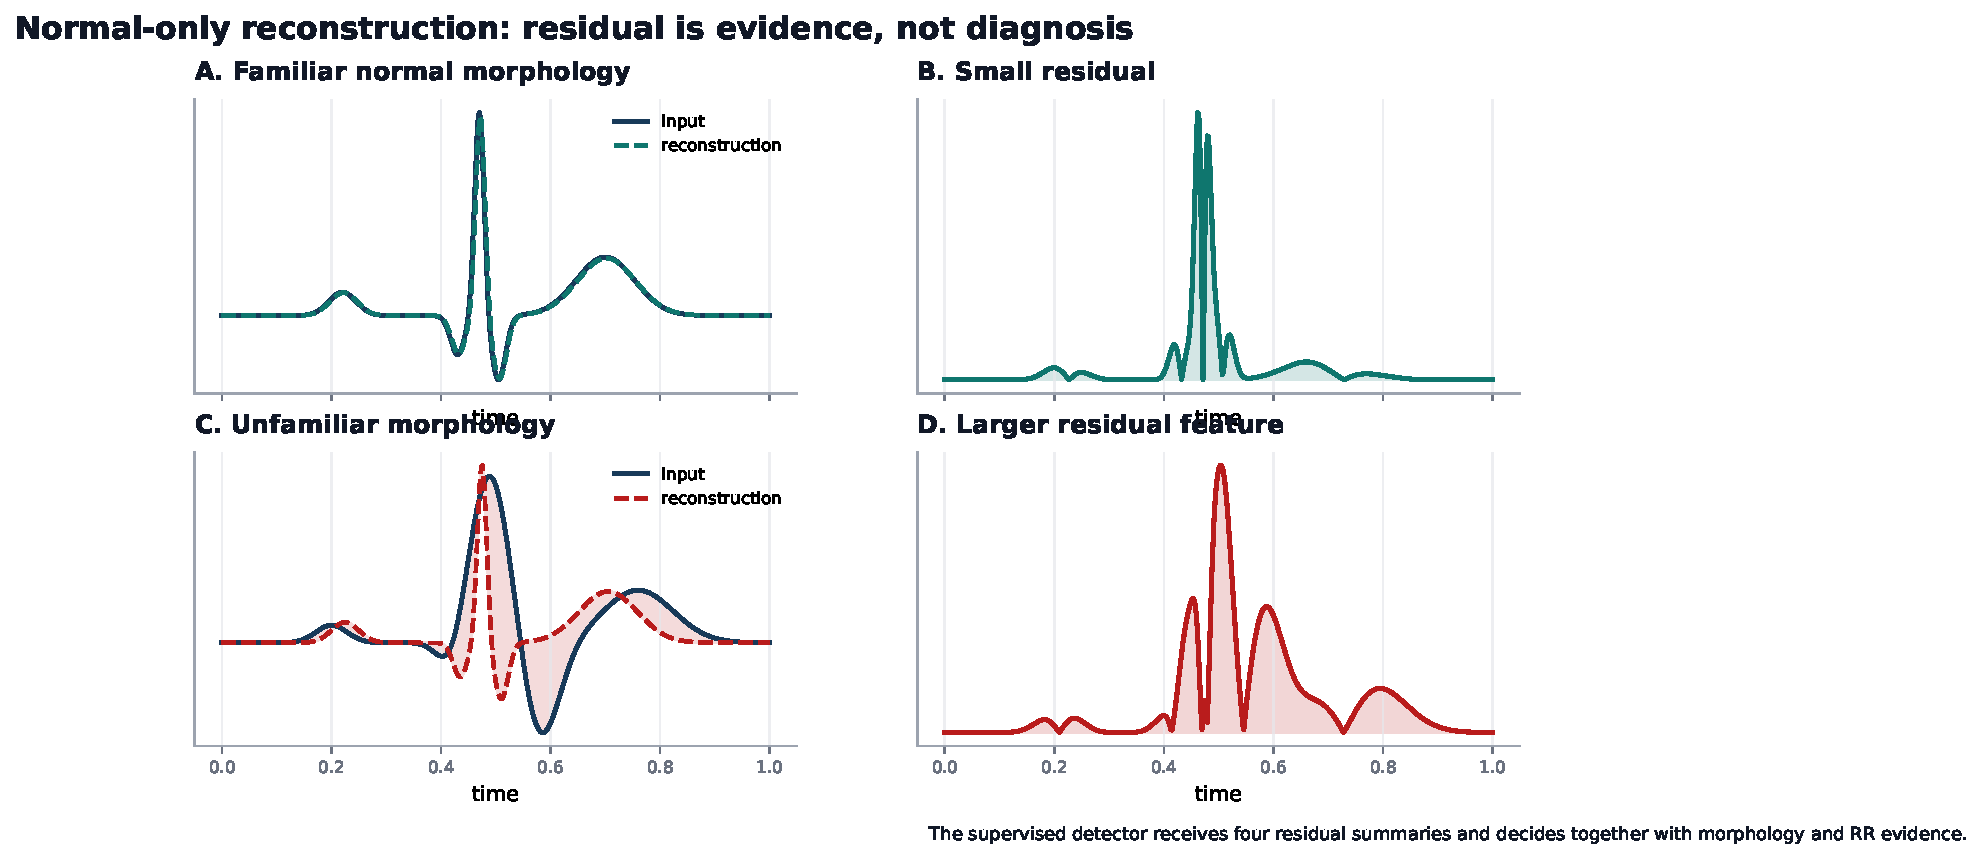
\includegraphics[width=0.92\textwidth,height=0.66\textheight,keepaspectratio]{theory_reconstruction_principle.pdf}

\figcaption{A larger residual may indicate novelty, but the final decision is
made by supervised tree models that also see MLII morphology and RR timing.}
\source{hinton2006autoencoder,vincent2008denoising,chandola2009anomaly}
\end{frame}

\begin{frame}{The hierarchy separates abnormality from subtype}
\centering
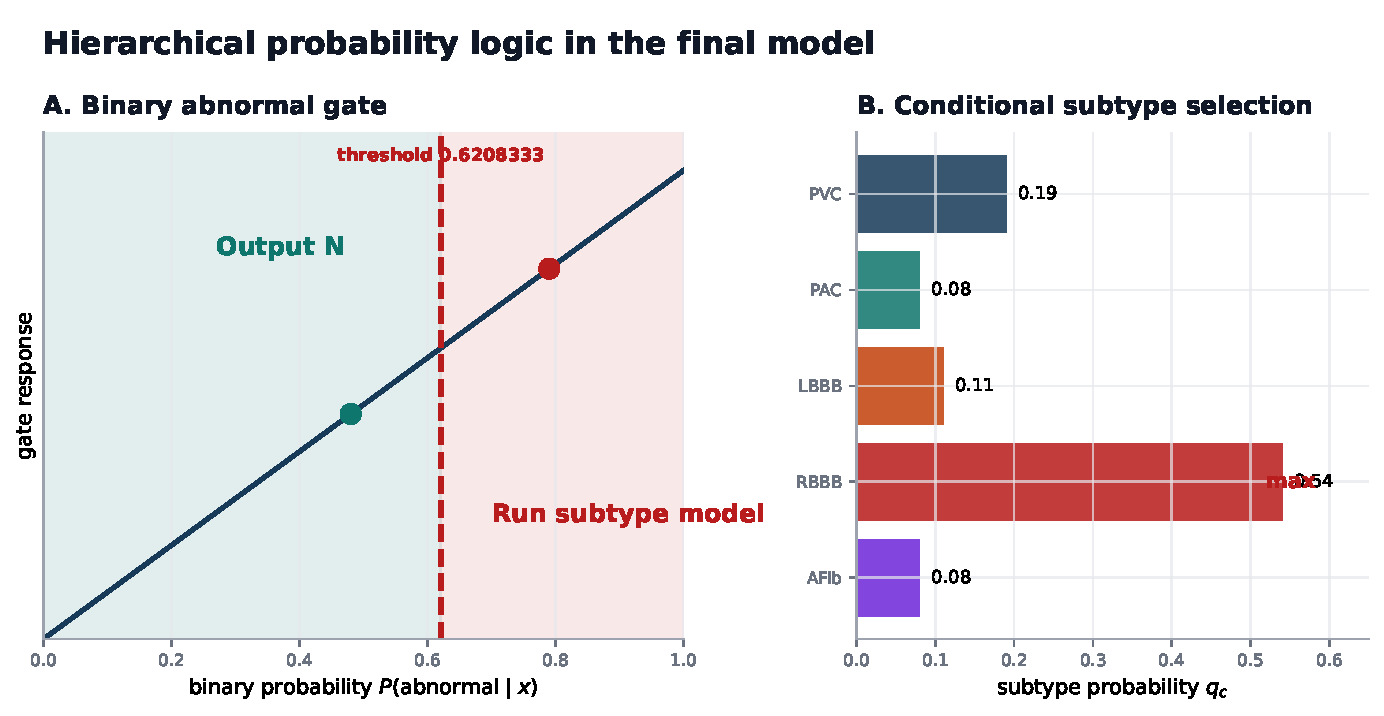
\includegraphics[width=0.91\textwidth,height=0.70\textheight,keepaspectratio]{theory_hierarchy_probability.pdf}

\figcaption{The subtype model is conditional: it is used only when the binary
gate passes the abnormality threshold.}
\end{frame}

\begin{frame}{Validation must respect patient clusters}
\centering
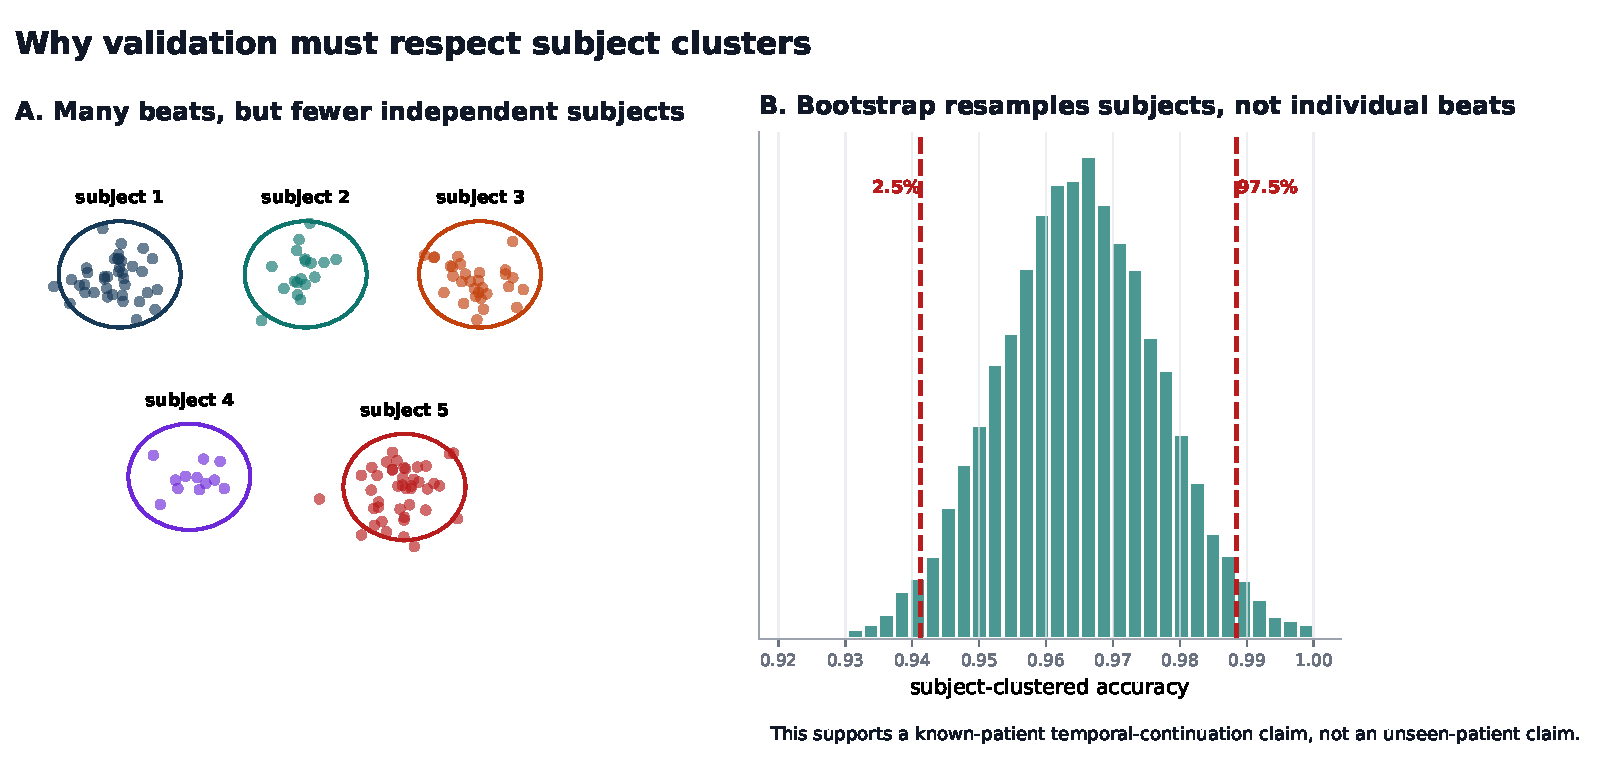
\includegraphics[width=0.92\textwidth,height=0.70\textheight,keepaspectratio]{theory_validation_units.pdf}

\figcaption{Subject-clustered resampling prevents many beats from one record
being treated as many independent people.}
\source{rutter2000clustered}
\end{frame}

\begin{frame}{The final runtime system is a one-lead hierarchy}
\centering
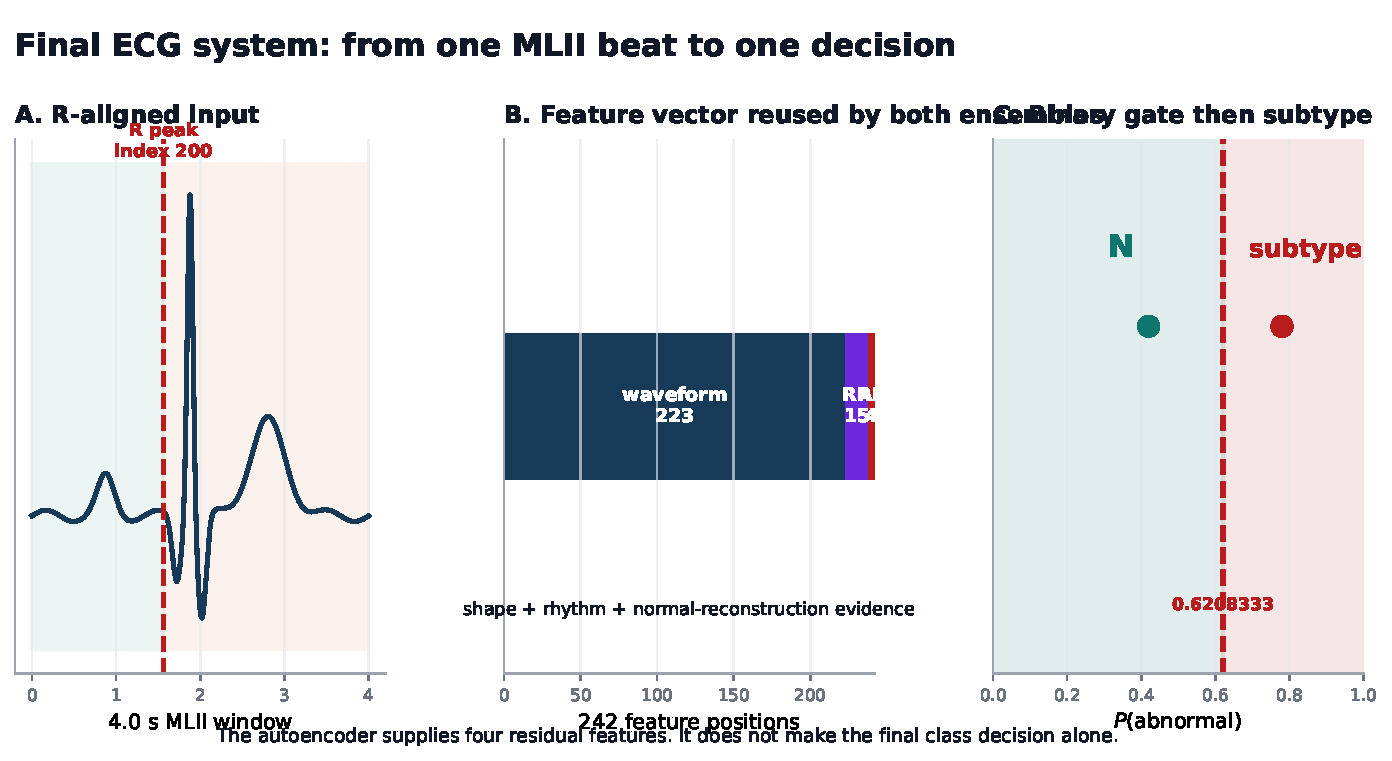
\includegraphics[width=0.94\textwidth,height=0.70\textheight,keepaspectratio]{architecture_current_system_flow.pdf}

\figcaption{For each detected MLII heartbeat, the saved system builds one
242-value vector, applies the abnormality gate, and conditionally applies the
five-class subtype model.}
\end{frame}

\begin{frame}{Each beat is scored from an R-aligned window}
\centering
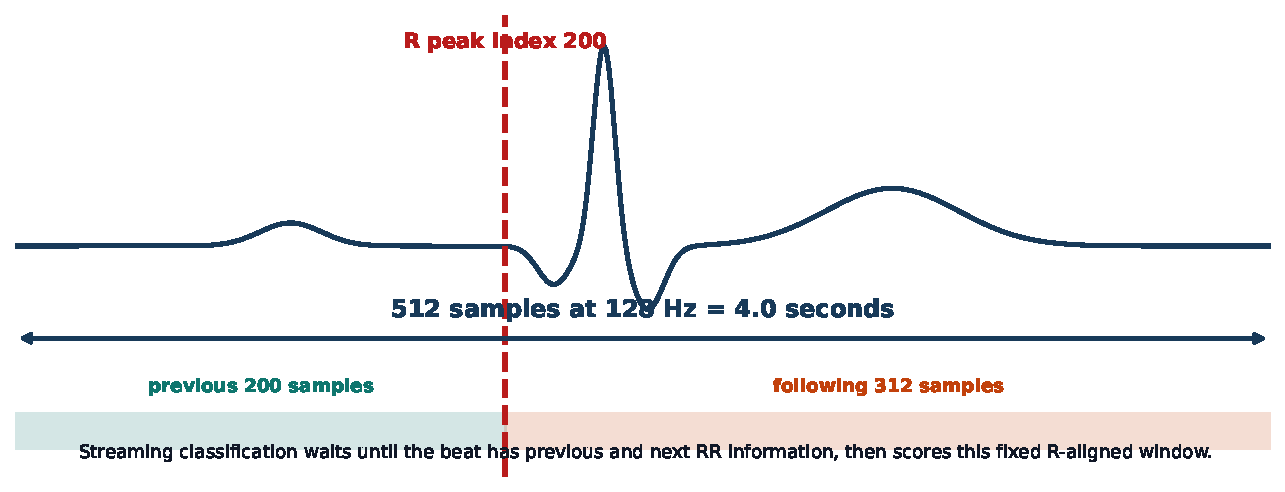
\includegraphics[width=0.90\textwidth,height=0.70\textheight,keepaspectratio]{architecture_streaming_window.pdf}

\figcaption{The R peak is fixed at sample index 200 inside a 512-sample,
four-second window, giving both pre-QRS and post-QRS context.}
\end{frame}

\begin{frame}{Training, testing, and installed use are separated}
\centering
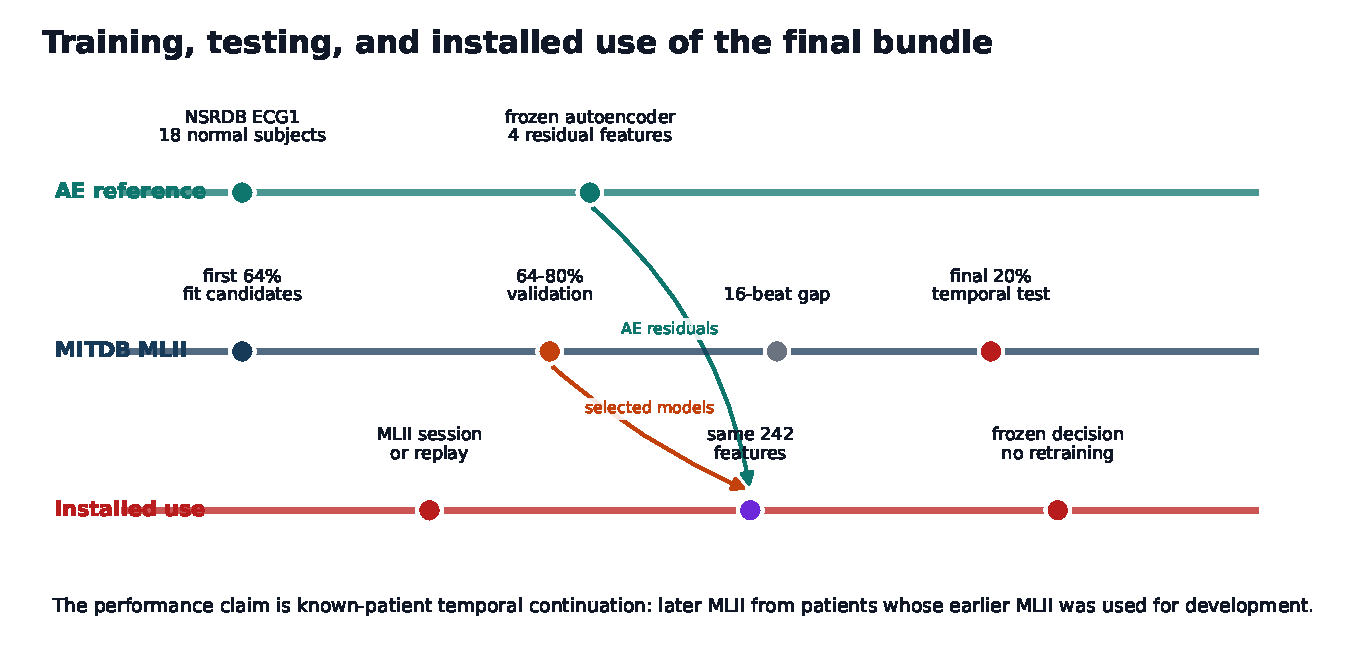
\includegraphics[width=0.94\textwidth,height=0.70\textheight,keepaspectratio]{architecture_training_live_map.pdf}

\figcaption{Live/session use applies the frozen bundle. It does not update the
autoencoder, the detector, or the subtype classifier.}
\end{frame}

\begin{frame}{The autoencoder checkpoint is frozen before supervised fitting}
\centering
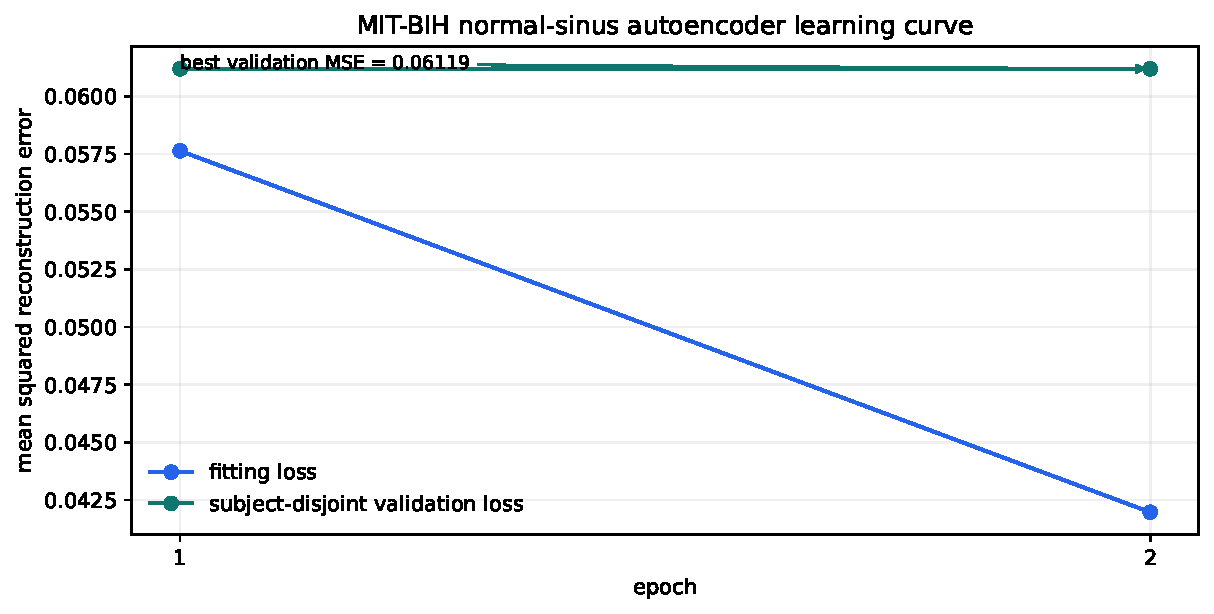
\includegraphics[width=0.80\textwidth,height=0.66\textheight,keepaspectratio]{nsrdb_autoencoder_learning_curve.pdf}

\figcaption{The normal-only autoencoder used 288,673 fitting windows from 15
NSRDB subjects and 57,177 validation windows from three different subjects.}
\end{frame}

\begin{frame}{Autoencoder mismatch becomes four residual features}
\centering
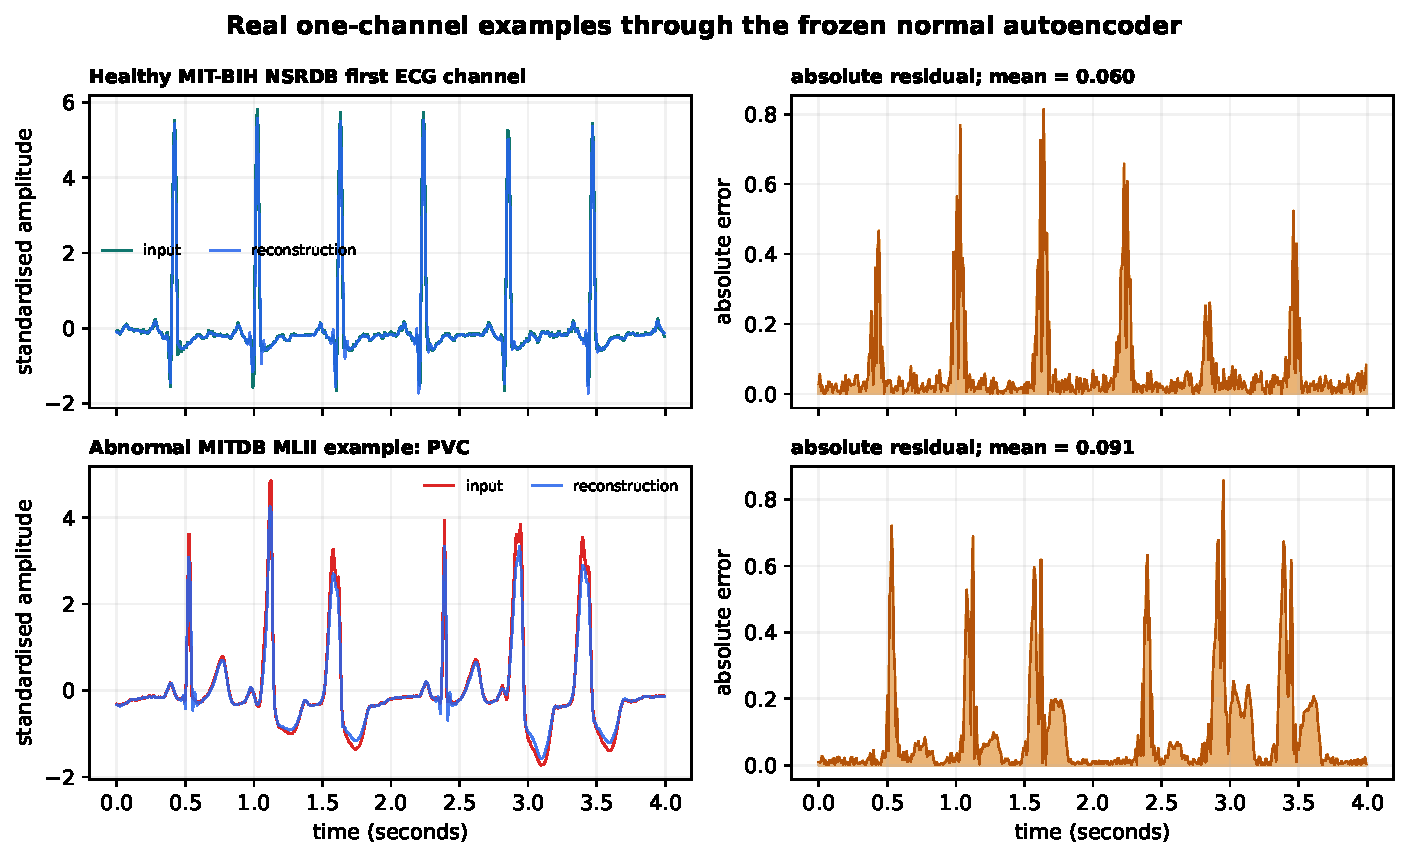
\includegraphics[width=0.92\textwidth,height=0.70\textheight,keepaspectratio]{real_autoencoder_processing.pdf}

\figcaption{Whole-window MAE, whole-window MSE, central morphology MAE, and
residual-change MAE are appended to the supervised feature vector.}
\end{frame}

\begin{frame}{Both supervised stages receive the same 242 values}
\centering
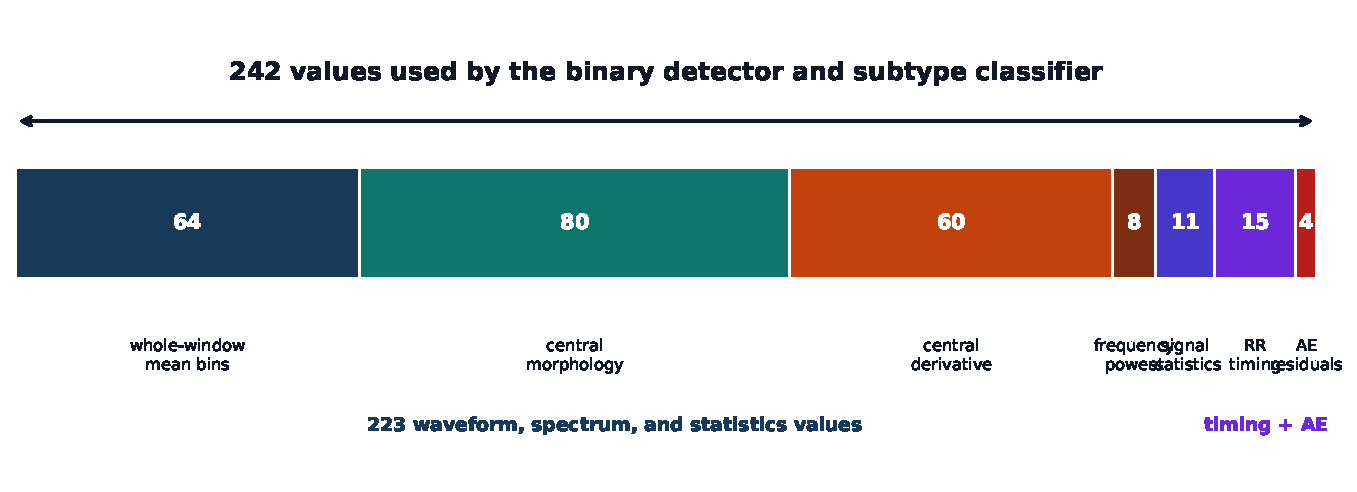
\includegraphics[width=0.94\textwidth,height=0.70\textheight,keepaspectratio]{architecture_feature_vector.pdf}

\figcaption{$223$ MLII waveform/statistical values, $15$ RR timing values, and
$4$ autoencoder residual values form the final evidence vector.}
\end{frame}

\begin{frame}{The final experiment keeps selection away from the test}
\centering
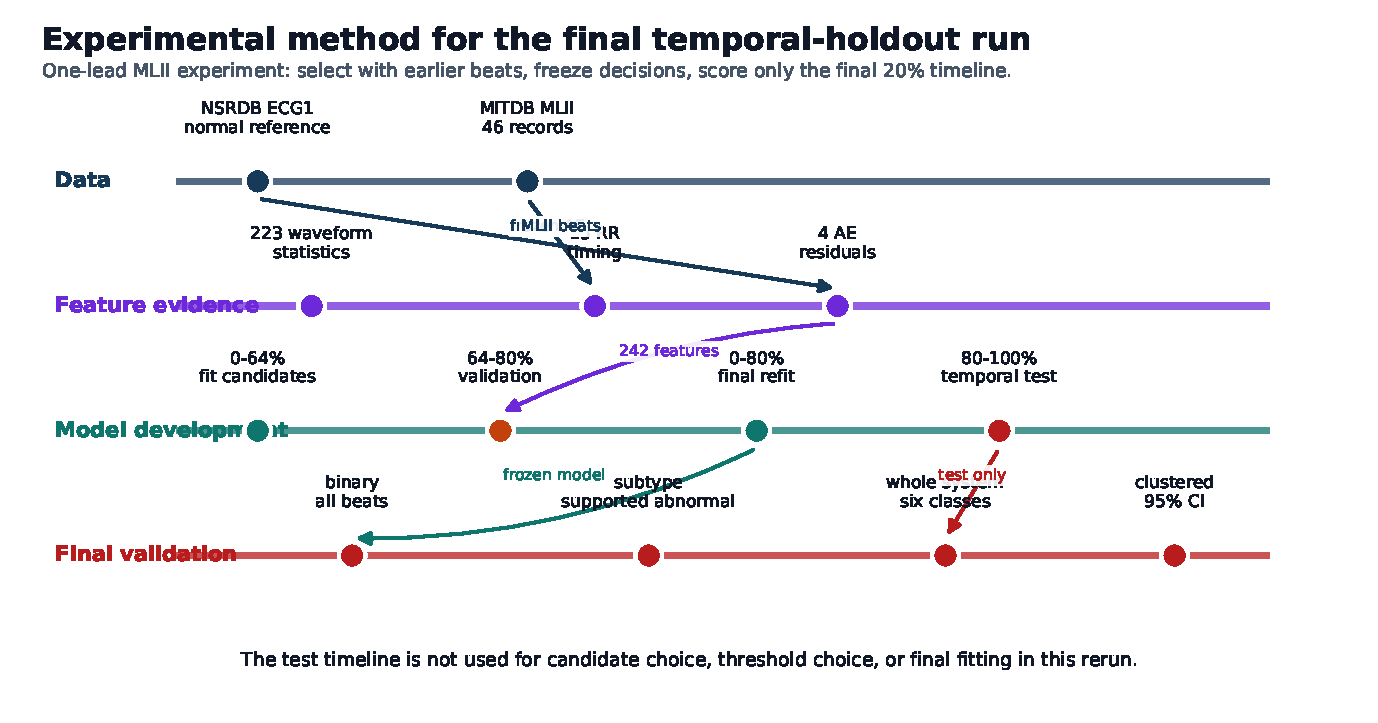
\includegraphics[width=0.93\textwidth,height=0.70\textheight,keepaspectratio]{method_final_workflow.pdf}

\figcaption{Candidate models are selected on earlier temporal regions, refit
before the test boundary, and scored only on the final 20\% timeline.}
\end{frame}

\begin{frame}{Every eligible record follows the same temporal split}
\centering
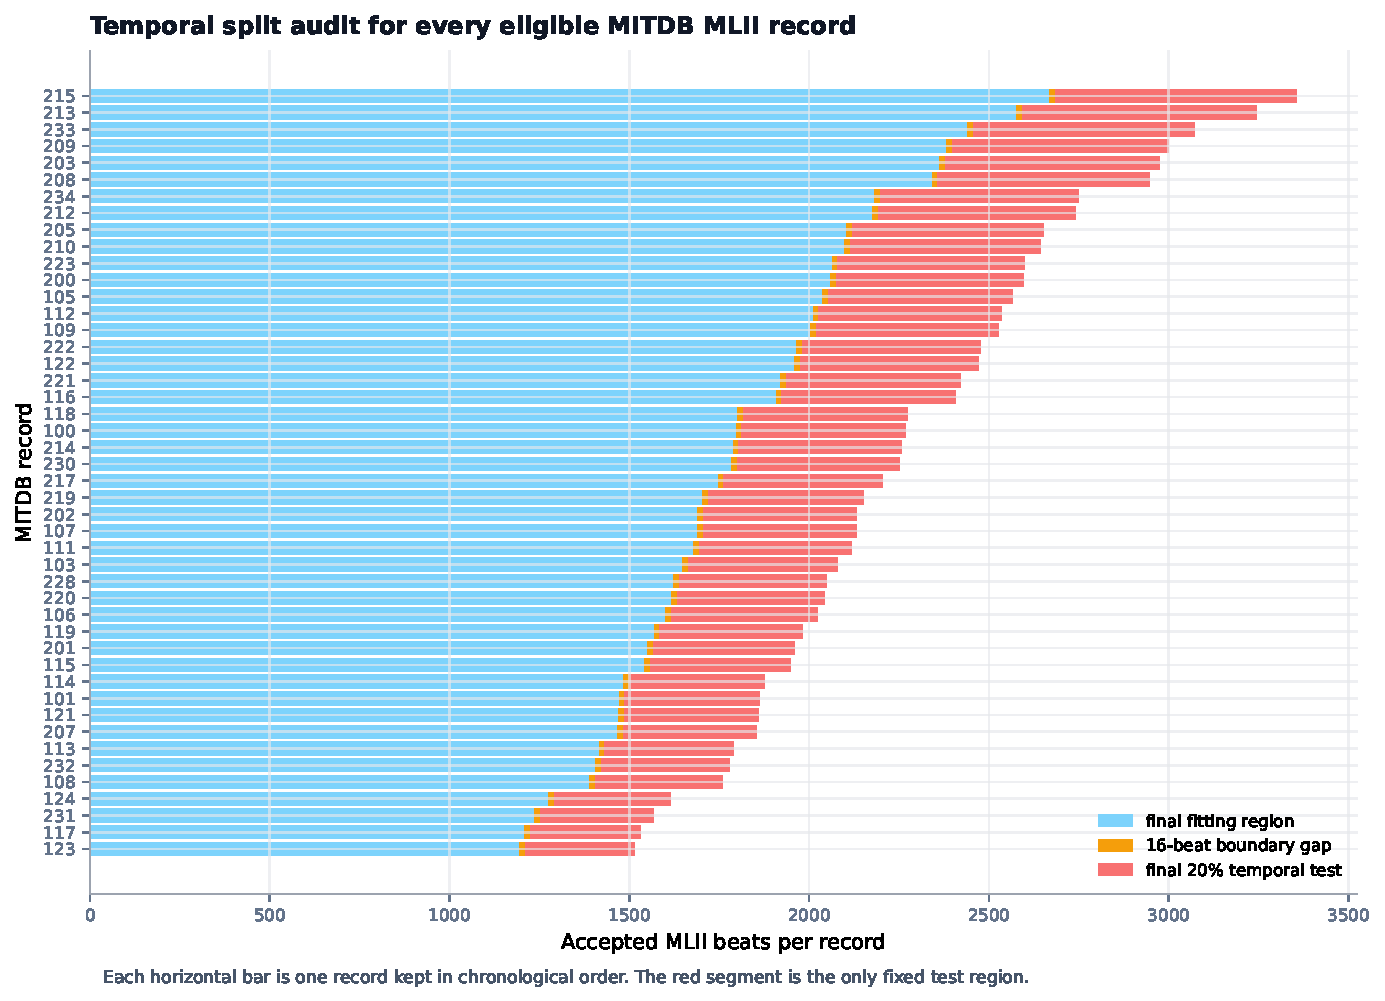
\includegraphics[width=0.94\textwidth,height=0.70\textheight,keepaspectratio]{method_temporal_split_audit.pdf}

\figcaption{Blue beats are available for final fitting, yellow beats are the
16-beat boundary gap, and red beats are the held-out final temporal test.}
\end{frame}

\begin{frame}{Validation selected the final Extra Trees pair}
\centering
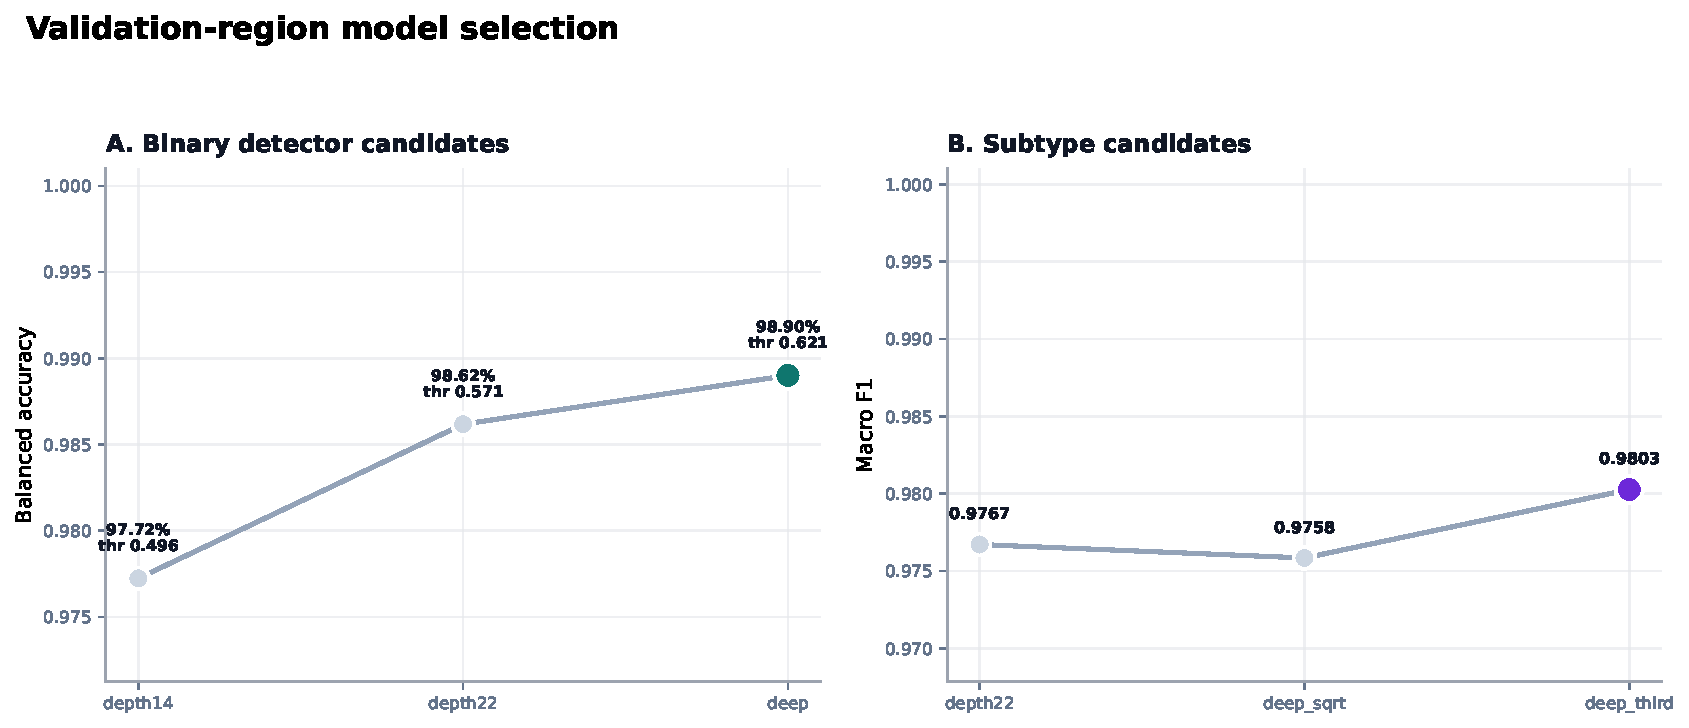
\includegraphics[width=0.91\textwidth,height=0.70\textheight,keepaspectratio]{method_model_selection.pdf}

\figcaption{The selected detector uses 240 trees and threshold 0.6208333. The
selected subtype model uses 260 trees with one-third feature sampling.}
\end{frame}

\begin{frame}{Three evaluations answer different questions}
\centering
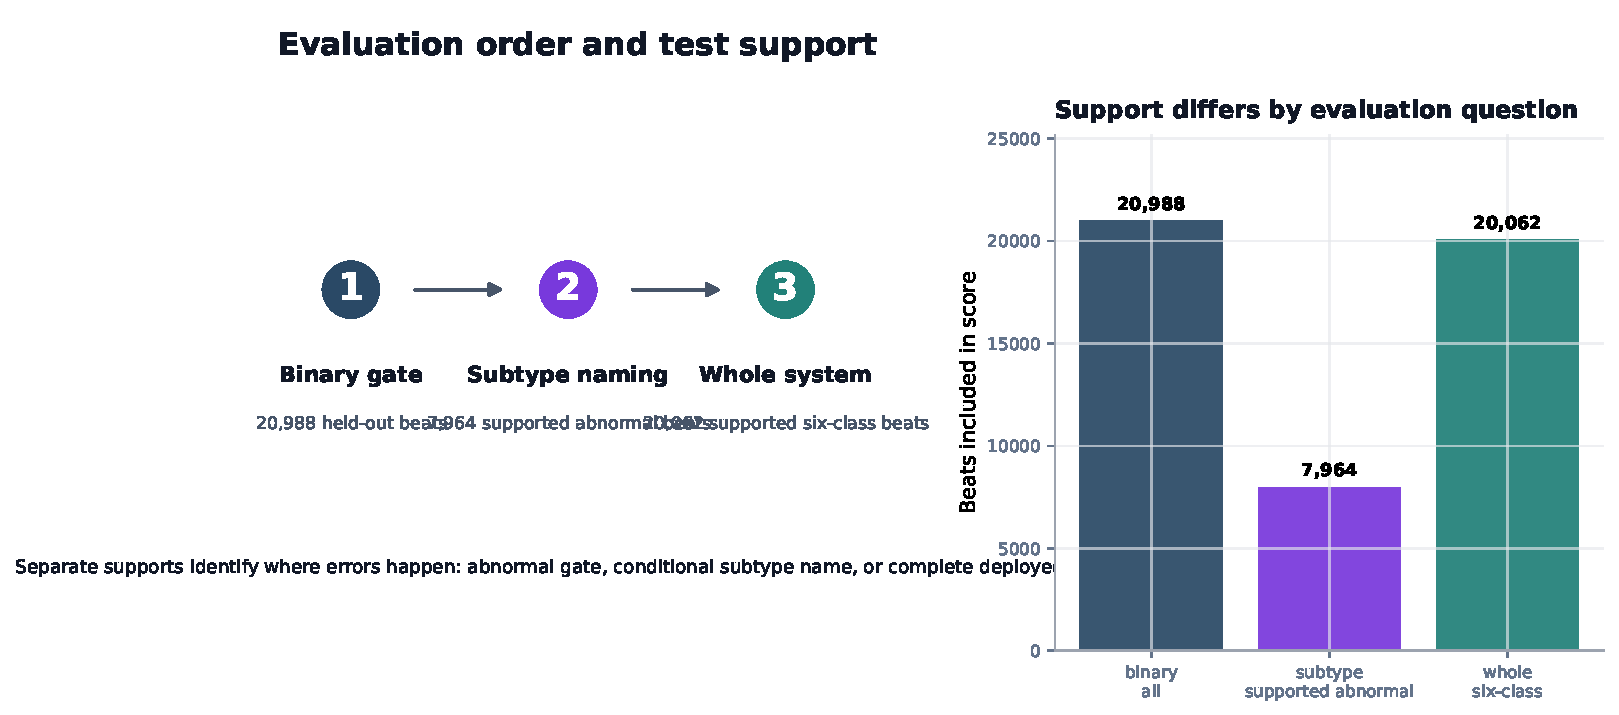
\includegraphics[width=0.92\textwidth,height=0.70\textheight,keepaspectratio]{method_evaluation_order.pdf}

\figcaption{Binary detection uses all held-out accepted beats. Conditional
subtype scoring uses true supported abnormal beats. Whole-system scoring uses
N plus the five supported abnormal classes.}
\end{frame}

\begin{frame}{The fixed test is later ECG from known patients}
\centering
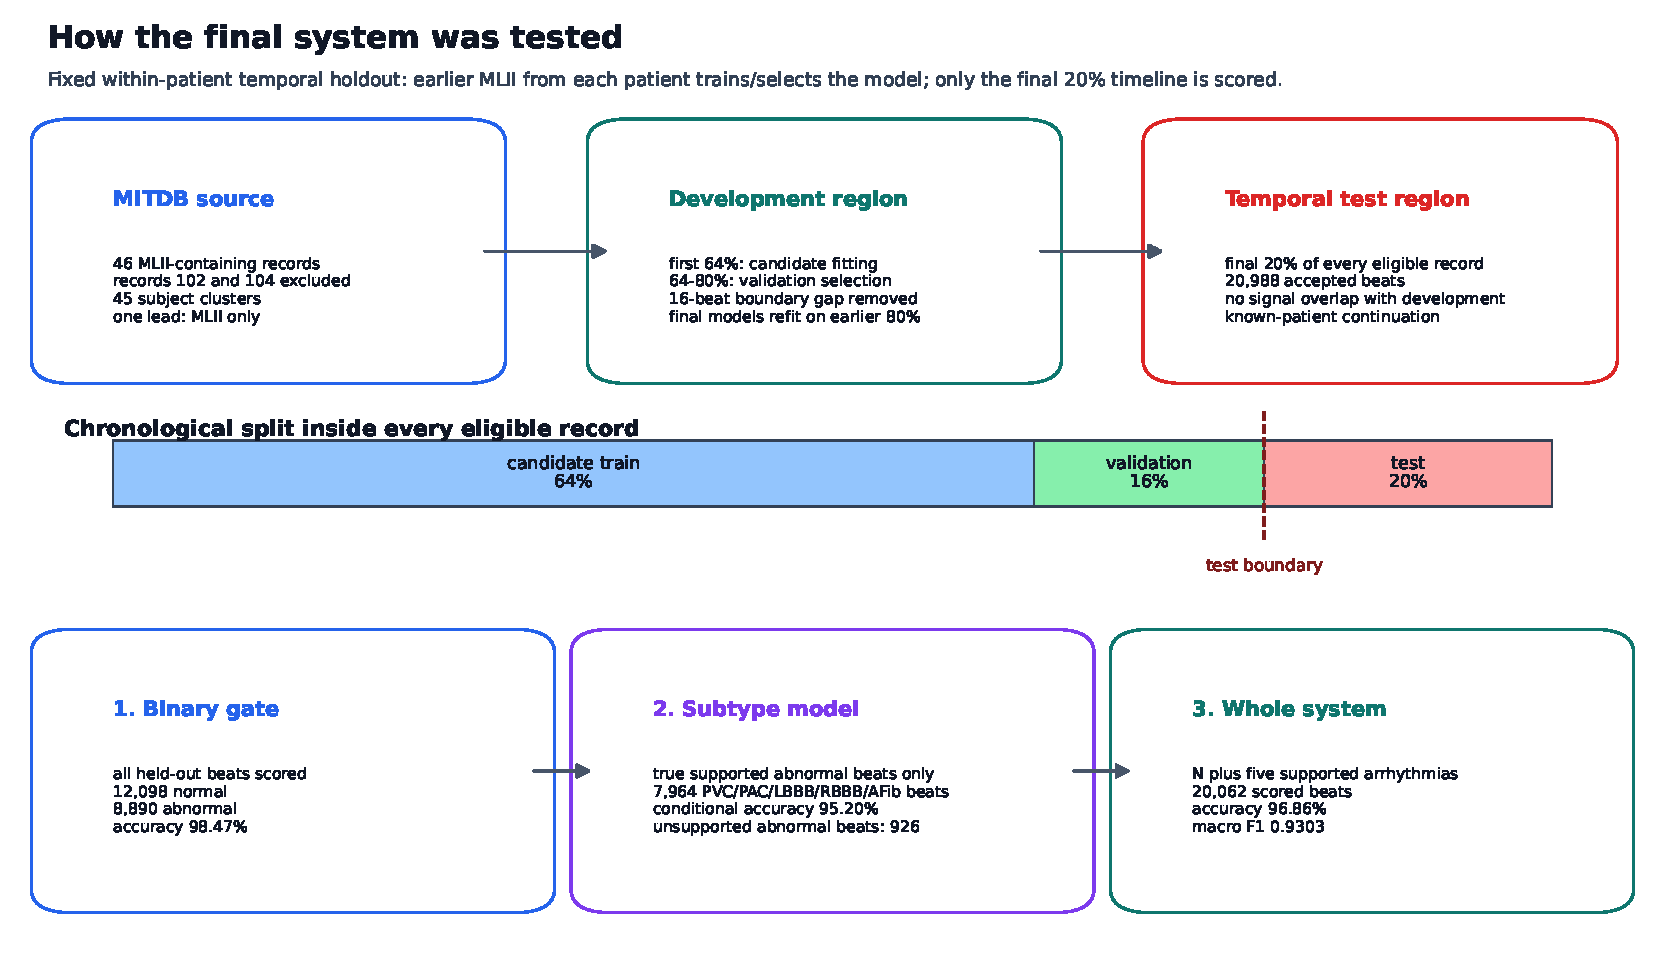
\includegraphics[width=0.93\textwidth,height=0.70\textheight,keepaspectratio]{final_testing_protocol.pdf}

\figcaption{The final 20\% of each eligible MITDB MLII record is held out for
scoring; earlier ECG from the same records remains available for development.}
\end{frame}

\begin{frame}{The whole-system test contains six supported outputs}
\centering
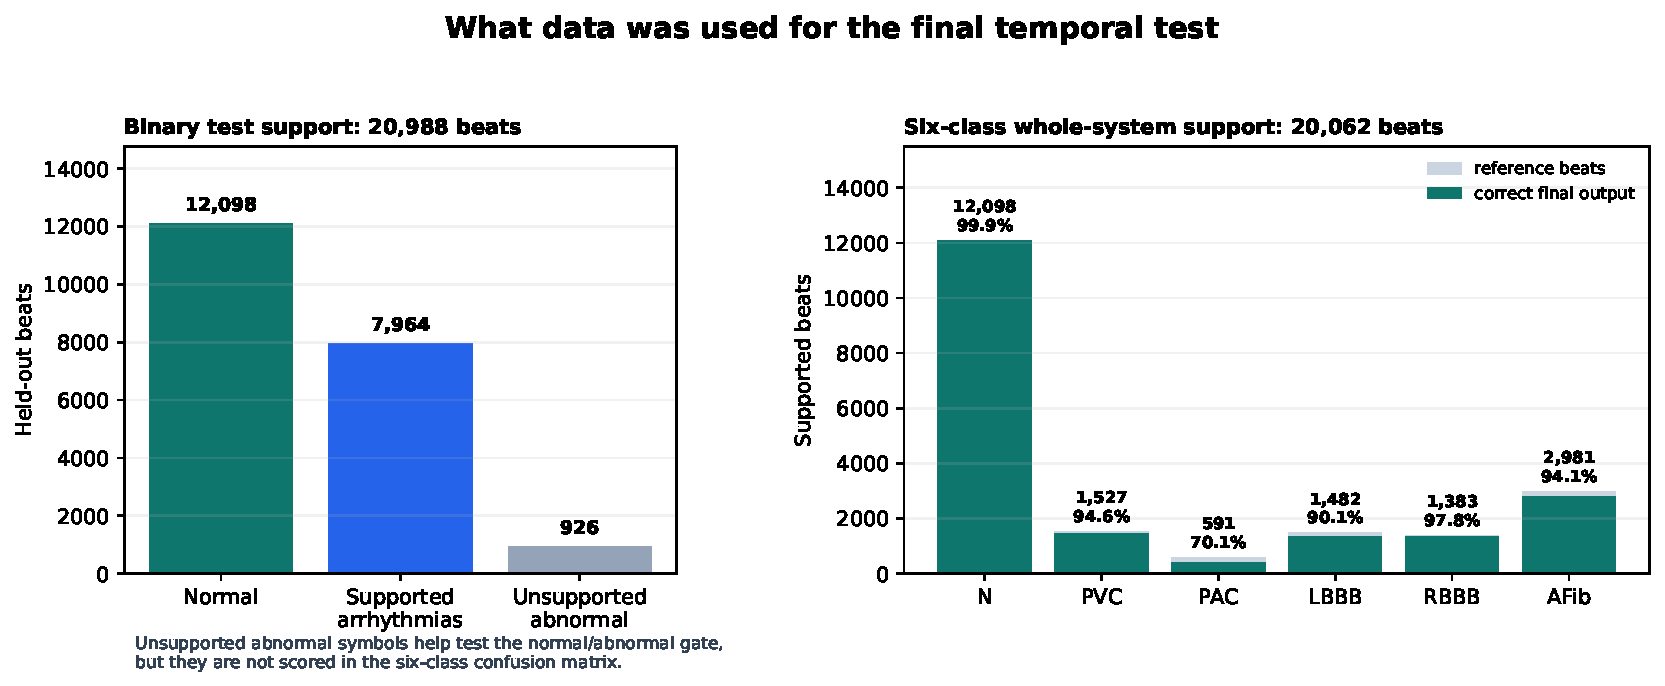
\includegraphics[width=0.93\textwidth,height=0.70\textheight,keepaspectratio]{final_test_composition.pdf}

\figcaption{The six-class whole-system test contains 20,062 supported beats:
N, PVC, PAC, LBBB, RBBB, and AFib. Unsupported abnormal beats remain in binary
testing only.}
\end{frame}

\begin{frame}{Temporal whole-system accuracy is 96.86\%}
\centering
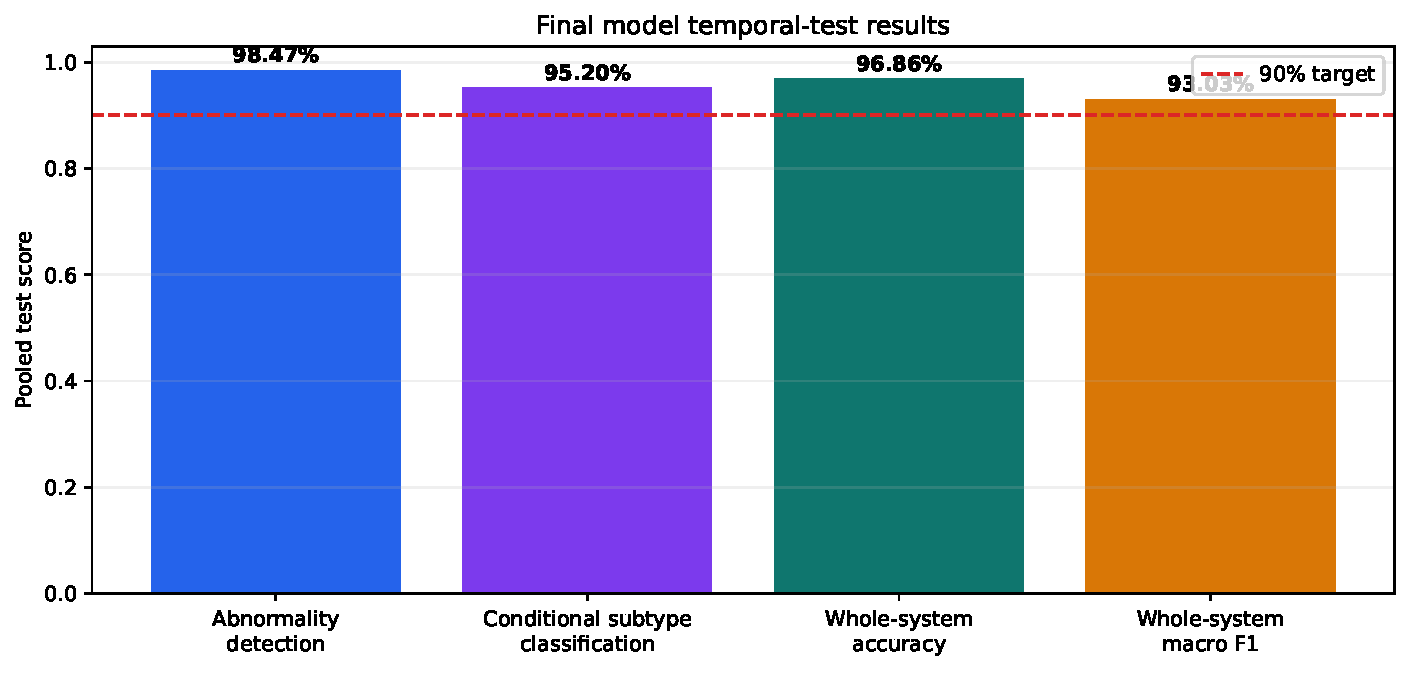
\includegraphics[width=0.82\textwidth,height=0.66\textheight,keepaspectratio]{final_metrics.pdf}

\figcaption{Binary accuracy is 98.47\%, conditional subtype accuracy is
95.20\%, whole-system accuracy is 96.86\%, and whole-system macro F1 is
0.9303.}
\end{frame}

\begin{frame}{The 95\% interval clears 90\%, but is still wide}
\centering
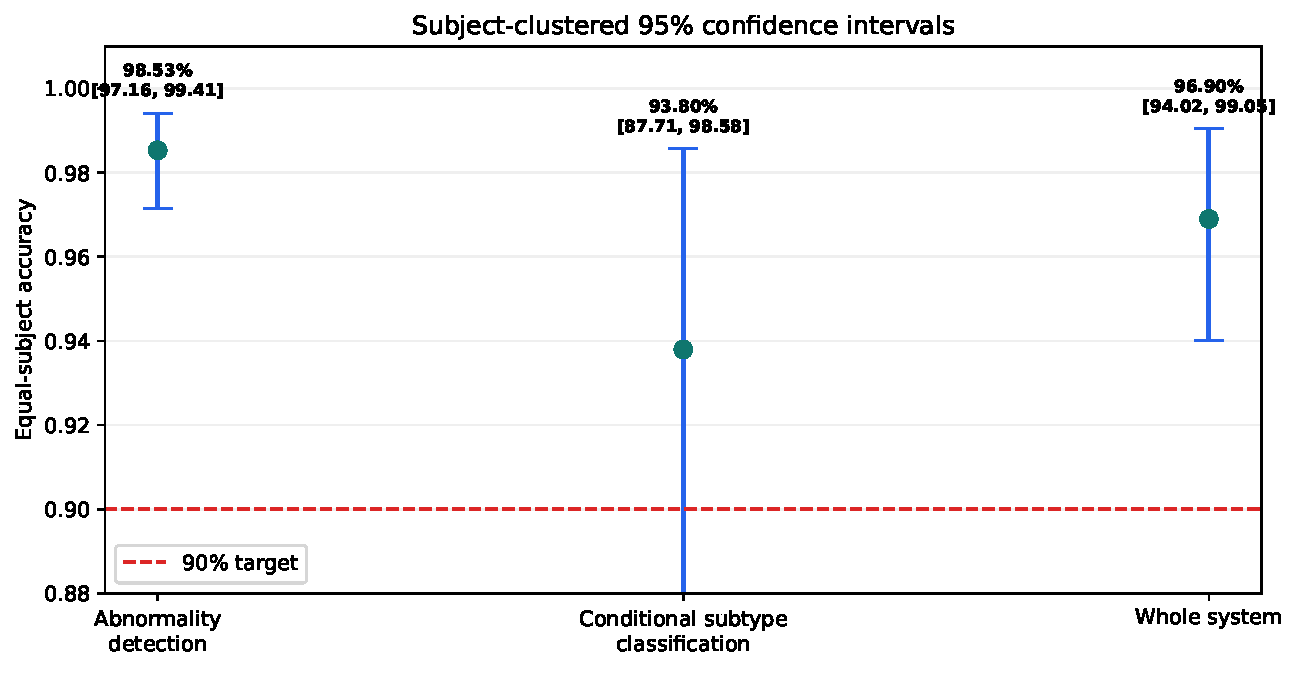
\includegraphics[width=0.80\textwidth,height=0.66\textheight,keepaspectratio]{final_clustered_ci.pdf}

\figcaption{Whole-system subject-clustered 95\% CI is 94.02--99.05\%. The
5.03-point width does not meet the planned three-point precision target.}
\end{frame}

\begin{frame}{Most subject clusters exceed the target}
\centering
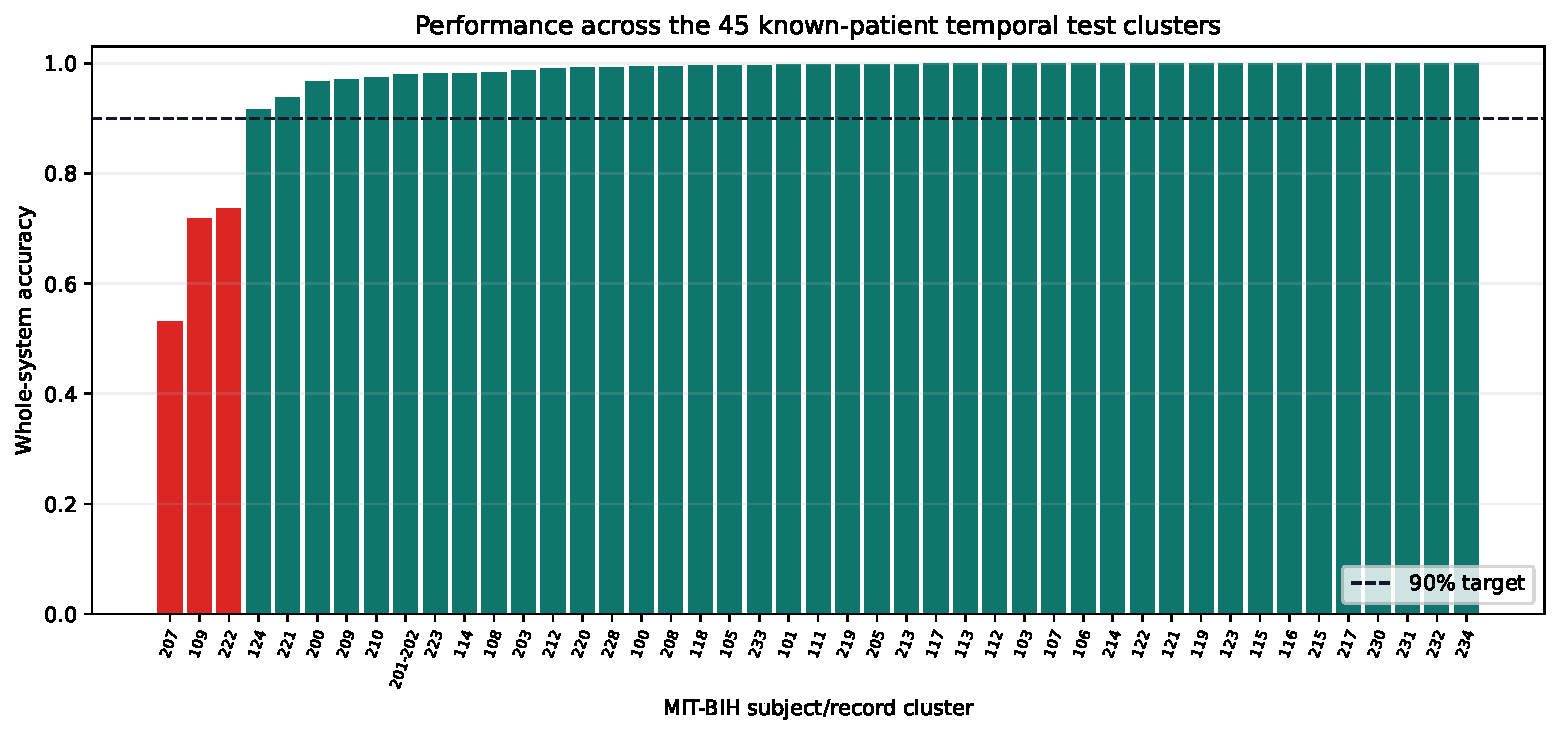
\includegraphics[width=0.94\textwidth,height=0.70\textheight,keepaspectratio]{final_subject_accuracy.pdf}

\figcaption{Forty-two of 45 subject clusters are above 90\%; equal-subject
whole-system accuracy is 96.90\%.}
\end{frame}

\begin{frame}{PAC is the main unsupported recall goal}
\centering
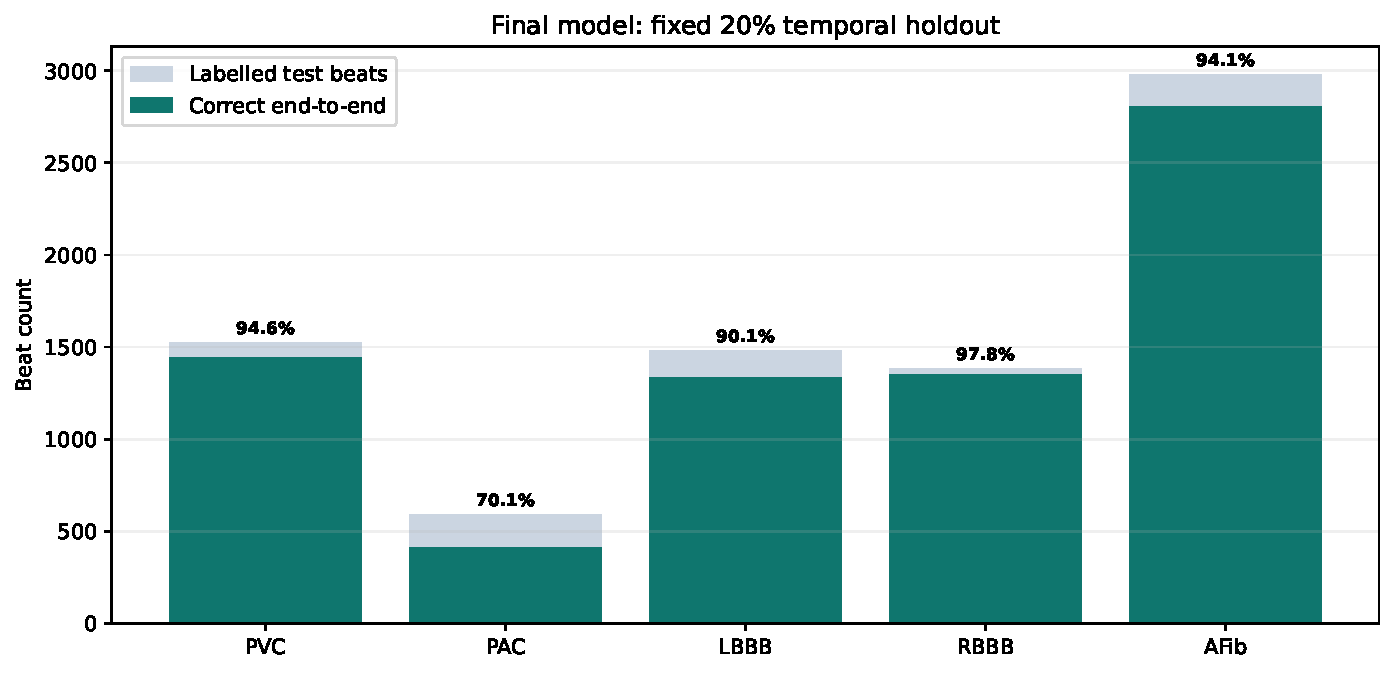
\includegraphics[width=0.86\textwidth,height=0.66\textheight,keepaspectratio]{final_arrhythmia_counts.pdf}

\figcaption{End-to-end recall is PVC 94.63\%, PAC 70.05\%, LBBB 90.15\%, RBBB
97.76\%, and AFib 94.13\%.}
\end{frame}

\begin{frame}{The confusion matrix shows the remaining failure modes}
\centering
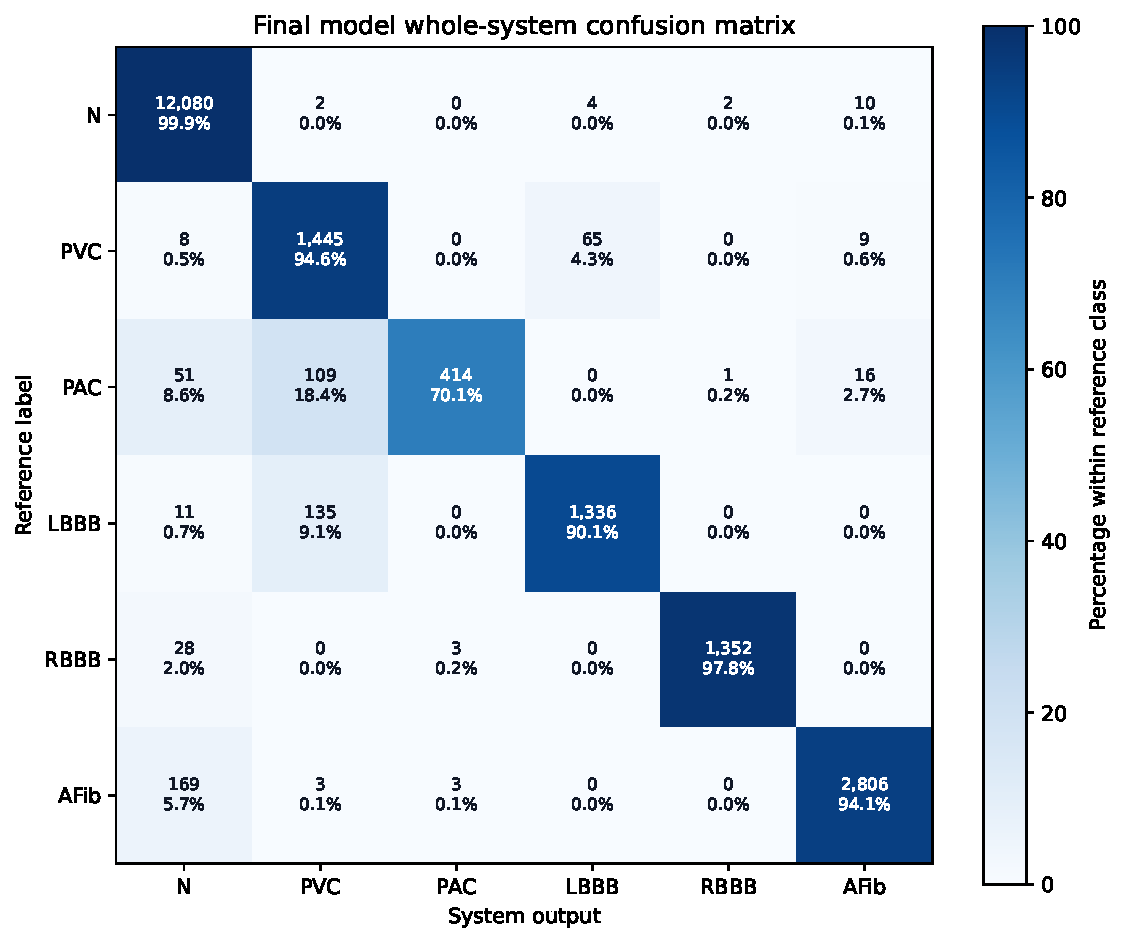
\includegraphics[width=0.78\textwidth,height=0.68\textheight,keepaspectratio]{final_confusion_matrix.pdf}

\figcaption{The largest subtype confusions are LBBB to PVC, PAC to PVC, and
PVC to LBBB. The binary gate also sends some AFib and PAC beats to normal.}
\end{frame}

\begin{frame}{The goals were reached only for the stated temporal scope}
\begin{description}
\item[Reached] Pooled whole-system accuracy exceeds 90\%.
\item[Reached] The subject-clustered lower 95\% bound exceeds 90\%.
\item[Not reached] Confidence-interval width is 5.03 rather than at most
three points.
\item[Not reached] PAC recall is 70.05\%, below 90\%.
\item[Not tested] Completely unseen patients or an external hospital database.
\end{description}
\vspace{0.2cm}
\begin{alertblock}{Safety conclusion}
This is a research prototype, not a clinical diagnostic device.
\end{alertblock}
\end{frame}

\begin{frame}{The next study must add independent patients}
\begin{enumerate}
  \item Keep the MLII input rule fixed across training and deployment.
  \item Add independent PAC, LBBB, RBBB, and AFib patients.
  \item Reserve an external patient-level database for one final test.
  \item Pre-register the lower CI bound, interval width, and per-class recall.
  \item Compare the full model with and without autoencoder residual features.
  \item Test real AD8232 recordings without changing the frozen model.
\end{enumerate}
\source{dechazal2004heartbeat}
\end{frame}

\begin{frame}{Final conclusion}
\begin{block}{Core finding}
A single ECG lead is sufficient for 96.86\% whole-system accuracy on unseen
later signal from known patients, with a subject-clustered 95\% interval of
94.02--99.05\%.
\end{block}
\begin{alertblock}{Required interpretation}
The result does not prove 96.86\% accuracy for a completely new patient. PAC
recall and interval width remain important weaknesses.
\end{alertblock}
\vspace{0.25cm}
The final software, experiment artifact, report, and presentation now describe
the same one-channel architecture, with MLII fixed for supervised use.
\end{frame}

\begin{frame}[allowframebreaks]{References}
\footnotesize
\bibliographystyle{ieeetr}
\bibliography{refe}
\end{frame}

\end{document}
